\subsection{Securización de las comunicaciones} \label{SegCom}
Para preservar la seguridad y privacidad en el protocolo de aprendizaje federado propuesto es imprescindible securizar las comunicaciones. Para securizarlas se han llevado a cabo dos acciones clave, la primera en lo que concierne al protocolo de comunicación y la segunda en cuanto al cifrado de la comunicación.

\subsubsection{Protocolo de comunicación}
En cuanto al protocolo de comunicación se ha optado por la utilización del protocolo SCP (Secure Copy Protocol), conocido en español como protocolo de copia segura. Este protocolo requiere del protocolo SSH (Secure Shell), conocido en español como terminal seguro.
\\ \\
El protocolo SSH permite el acceso remoto a un servidor o dispositivo por un canal seguro a través de una clave. Además, el protocolo usa técnicas de cifrado que impiden que la información que viaje en la red lo haga de forma legible. El protocolo SCP permite la transferencia de archivos entre dispositivos de la red usando el protocolo SSH como base.

\subsubsection{Cifrado de la comunicación}
Aunque las comunicaciones en el protocolo SCP y SSH vayan cifradas son susceptibles de ser atacadas. Para mejorar este aspecto se ha realizado un sistema de cifrado de los modelos que viajen por la red para preservar la privacidad y seguridad de los participantes.
\\ \\ 
Para esta labor se han utilizado el método criptográfico de criptografía híbrida, que usa tanto la criptografía simétrica como asimétrica.

\paragraph{Cifrado simétrico} 
El cifrado simétrico es aquel sistema de cifrado en el que la misma clave sirve para cifrar como para descifrar el mensaje. 
\\ \\
El problema de este sistema es que toda la seguridad reside en la clave empleada en el cifrado. Esto es un gran impedimento a la hora de gestionar comunicaciones debido al cómo gestionar el envío de esta clave, ya que si no se hace por un canal seguro el mensaje sera fácilmente descifrable.
\\ \\
Por otro lado, este sistema cuenta con dos grandes ventajas, es sencillo, es rápido y requiere menos recursos para llevarlo a cabo.

\paragraph{Cifrado asimétrico}
El cifrado asimétrico es aquel sistema de cifrado que consta de dos claves criptográficas, una pública y una privada. La clave pública es utilizada para cifrar el mensaje mientras que la privada es utilizada para descifrarlo. 
\\ \\
Este sistema cuenta con tres grandes desventajas que impiden su uso en exclusivo o su uso con grandes volúmenes de información a cifrar. 
\begin{itemize}
    \item Se necesita más procesado de computo para generar la clave.
    \item Las claves asimétricas son mucho más grandes que las simétricas.
    \item El mensaje cifrado ocupa más espacio que el original.
\end{itemize}

Debido a que los dispositivos con los que se cuenta no tienen una gran capacidad de computo no se podría establecer un tamaño de clave lo suficientemente grande como para poder cifrar el modelo de inteligencia artificial completo. Este modelo pesa al rededor de los 7Kb y para cifrarlo con este sistema habría que generar una clave del mismo tamaño mayor.
\\ \\
Sin embargo, este sistema al constar de dos claves independientes es más sencillo salvaguardar la privacidad y seguridad de los integrantes.

\paragraph{Cifrado híbrido}
Teniendo en cuenta los anteriores dos tipos de cifrado se decidió utilizar el sistema híbrido para obtener los resultados más óptimos, protegiendo la privacidad y pudiendo realizar las tareas de cifrado desde dispositivos con menor capacidad computacional.
\\ \\ 
El proceso de cifrado se ha realizado de acorde al diagrama de flujo representado en la figura \ref{fig:Flow_Encryption}. En este diagrama se pueden observar los pasos que se han realizado para la encriptación de la información, en primer lugar el modelo de LightFM se convertió a bytes y se comprimió para reducir el volumen de datos a enviar por la red, pudiendo agilizar así las comunicaciones. Después se cifró simétricamente, generando una clave y un mensaje cifrado. Por un lado este mensaje cifrado sería comprimido y se guardaría en un fichero para su posterior envío. Por otro lado, la clave de cifrado simétrica se encriptó asimetricamente con la clave pública del receptor del mensaje, dando como resultado una clave de cifrado simétrico cifrada asimetricamente. Esta clave sería guardada en un fichero para ser enviada al igual que el mensaje.
\begin{figure}[H]
    \centering
    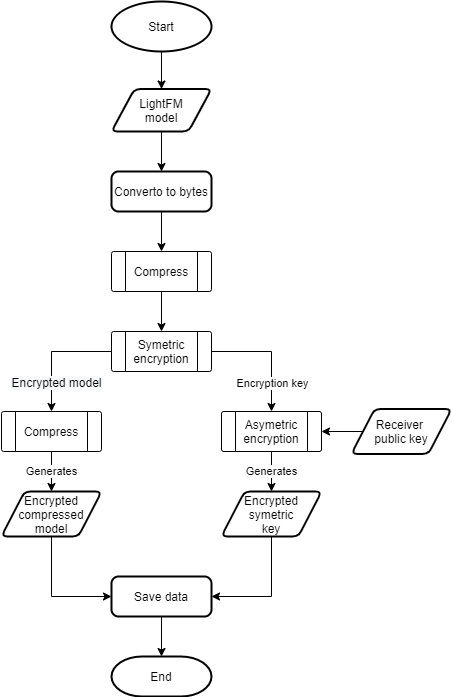
\includegraphics[height=0.6\textheight]{Figuras/flowchart_encryption.png}    
    \caption{Diagrama de flujo del proceso de cifrado} 
    \label{fig:Flow_Encryption}
\end{figure}


\subsubsection{Descifrado del mensaje}
El descifrado del mensaje es el proceso inverso al cifrado de la figura \ref{fig:Flow_Encryption}. Para ello, en un primer momento se reciben tanto el modelo cifrado simétricamente como la clave del modelo cifrada asimétricamente. En primer lugar, la clave que se ha recibido se descifra asimétricamente con la clave privada propia, ya que esta solo es descifrable por el receptor. Una vez descifrada la clave, se descomprime el modelo y se descifra con esta. Por último, el resultado es descomprimido y convertido a objeto LightFM para su posterior utilización. 
\begin{figure}[H]
    \centering
    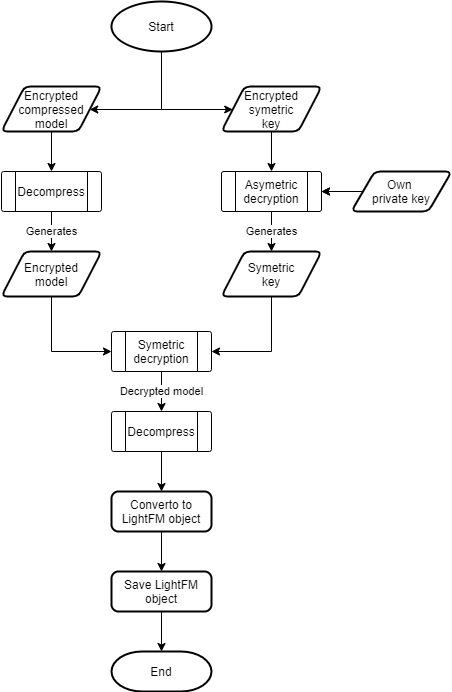
\includegraphics[height=0.6\textheight]{Figuras/flowchart_decryption.png}    
    \caption{Diagrama de flujo del proceso de descifrado} 
    \label{fig:Flow_Decryption}
\end{figure}